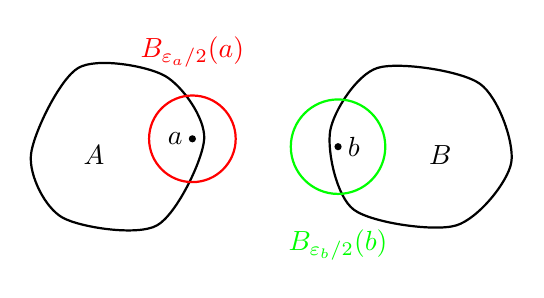
\begin{tikzpicture}[scale=1]
\draw[thick] plot[smooth cycle] coordinates {(-3,0) (-2.4,1.1) (-1.3,1.0) (-0.8,0.2) (-1.4,-0.9) (-2.6,-0.8)};
\node at (-2.2,0) {$A$};
\draw[thick] plot[smooth cycle] coordinates {(0.8,0.3) (1.4,1.1) (2.7,0.9) (3.1,-0.1) (2.4,-0.9) (1.1,-0.7)};
\node at (2.2,0) {$B$};
\fill (-0.95,0.2) circle (1.3pt) node[left] {$a$};
\draw[red, thick] (-0.95,0.2) circle (0.55);
\node[red] at (-0.95,1.3) {$B_{\varepsilon_a/2}(a)$};
\fill (0.9,0.1) circle (1.3pt) node[right] {$b$};
\draw[green, thick] (0.9,0.1) circle (0.6);
\node[green] at (0.9,-1.15) {$B_{\varepsilon_b/2}(b)$};
\end{tikzpicture}
